\documentclass[10pt]{myNSF}

\usepackage{amssymb}
\usepackage{graphicx}
\usepackage{wrapfig}
\usepackage{natbib}
\usepackage{url}
\usepackage{mdwlist}
\usepackage{aastex_macros}
\usepackage{mypack}
\usepackage{comment}

\begin{document}

\section{Project Description: New Wide-band Digital Technology and
  Interference Excision for Radio Astronomy}
\label{sec:project_description}

\subsection{Overview}
\label{sec:overview}

Advances in radio frequency (RF) analog and digital devices are
opening new possibilities for ultra-wide bandwidth (UWB) radio
astronomy science.  However, a complete UWB digital signal processing
(DSP) system that takes advantage of these advances is not yet
available.  UWB instrumentation also poses new challenges for sharing
the spectrum with other users.  We therefore propose to research and
develop new technologies and techniques for UWB radio astronomy, and
for maintaining the highest data quality in the presence of
terrestrial radio frequency interference (RFI).  Our project consists
of four main activities:
\vspace{-1em}
\begin{enumerate*}
\item{Develop the hardware, firmware, and tool flows needed to
  integrate cutting-edge analog to digital converters (ADCs) and field
  programmable gate arrays (FPGAs) for radio astronomy applications.
  \emph{The primary outcome of this activity will be the next
    generation of UWB DSP boards and a prototype system for the Robert
    C.\ Byrd Green Bank Telescope (GBT).}}
\item{Create standard, quantitative, and well-tested procedures for
  validating real-time RFI excision techniques and ensuring that they
  preserve scientific data quality, for use in this project and as a
  service to the community. \emph{The primary outcome of this activity
    will be tools and best practices that are necessary for testing
    the efficacy of RFI excision algorithms and building confidence in
    their use among scientists.}}
\item{Develop new algorithms for identifying and removing RFI in
  real-time, validate them using the procedures created in activity
  two, and implement them in our UWB DSP system.  \emph{The primary
    outcome of this activity will be innovative RFI excision
    techniques, ready to be used by radio astronomy observatories in
    the US and around the world.}}
\item{Engage first-generation college students in STEM fields through
  a two-week summer internship at the Green Bank Observatory (GBO),
  during which they will directly contribute to the RFI excision work
  by helping to create a public database of common RFI. This
  internship will leverage GBO's partnership in the NSF-INCLUDES
  program.  \emph{The primary outcome of this activity will be a
    cohort of students that are better prepared for STEM careers.}}
\end{enumerate*}
\vspace{-1em} The majority of this work will be conducted at GBO, in
close collaboration with the University of California, Berkeley (UCB)
and as part of the Collaboration for Astronomy Signal Processing and
Electronics Research (CASPER).  Through CASPER, we will ensure that
the outcomes of our work are shared broadly.  \emph{As a
  Federally-Funded Research and Development Center, GBO has been
  granted an exemption by NSF to submit this proposal since the
  resulting technical innovations will make unique contributions to
  the needs of researchers across the scientific community.}  GBO
staff have proven expertise in taking research projects from concept
to design and construction with a goal of repeatable, reliable,
maintainable, and scalable production use.  By operating the GBT and
other site telescopes, and working within the National Radio Quiet
Zone (see Facilities, Equipment, and other Resources), GBO staff have
gained unique experience in how to identify, assess, and mitigate RFI.
%We will also employ rigorous systems engineering to ensure that the
%products of our research can be easily deployed for future use.

This project is the first step in a longer-term effort to build a next
generation, end-to-end DSP system and flexible digital back-end for
the GBT that employs active RFI mitigation.  Such a system would be
used to maximize scientific return of a new UWB radio receiver under
independent development by GBO, and could also be adapted for use at
other observatories.  We will also lay the ground-work for
revolutionary upgrades to the GBT that will expand its available
bandwidth (BW) and enhance performance across all areas of radio
astronomy science.

We describe the motivation for this project in more detail in
\S\ref{sec:motivation}, and specify the innovative work that we will
carry out in \S\ref{sec:innovation}.  In \S\ref{sec:commitment} we
affirm our commitment to making the results of this project of broad
use, and in \S\ref{sec:infrastructure} we explain how the outcomes of
our work can be applied to enhance research at GBO, and at other US
and world observatories.  We describe our two-week STEM student
internship program in \S\ref{sec:workforce}.  We explain our timeline
and how the project will be managed to ensure success in
\S\ref{sec:management}.

\subsection{Intellectual Merit}
\label{sec:intellectual_merit}

\subsubsection{A Review of Existing Technology and Equipment}
\label{sec:review}

\begin{figure}
  \centering 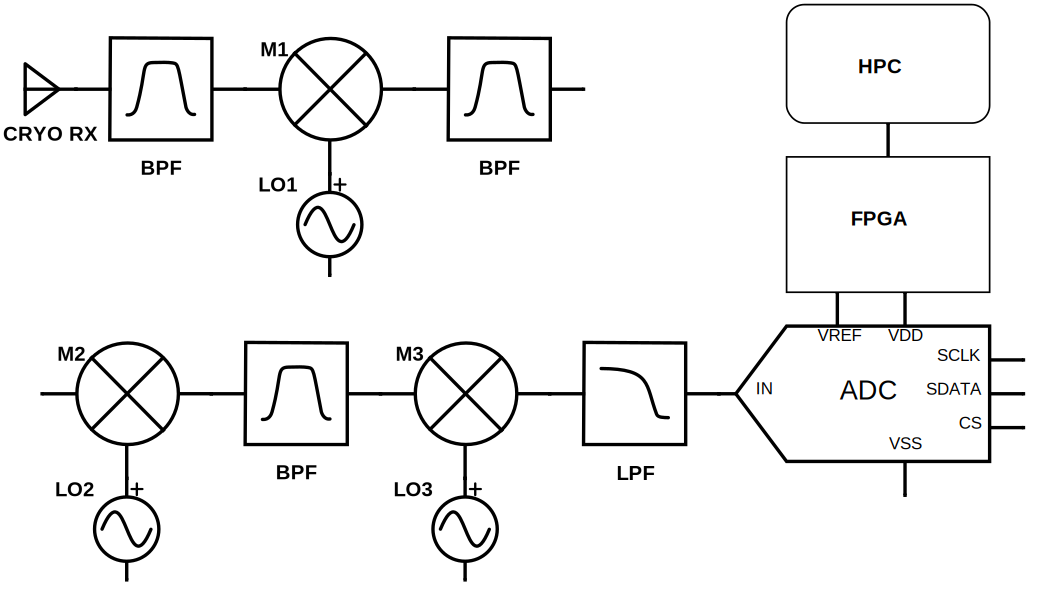
\includegraphics[width=0.9\textwidth]{if_diagram.png}
  \caption{A simplified block diagram representation of the existing
    GBT intermediate frequency system.  Components in the ``receiver
    room'' are located next to the radio receivers on the GBT.
    Signals are transported via IF-over-fiber (dashed line) to the
    ``equipment room'', which houses additional analog and digital
    instruments. Only one polarization channel is shown.  Individual
    receivers will have slightly different
    configurations. \label{fig:gbt_if}}
\end{figure}
  
We begin by reviewing the existing instrumentation for wide-bandwidth
radio astronomy using the GBT as an example.  The GBT is the world's
largest fully-steerable telescope and offers nearly continuous
coverage from $0.3$--$116\; \GHz$ (excepting the $50$--$67\; \GHz$
oxygen absorption band).  The Versatile Green Bank Astronomical
Spectrometer (VEGAS, developed with support from NSF award
AST-1006509) is the current primary digital back-end instrument.
VEGAS employs eight CASPER ROACH2 boards, each equipped with two 8-bit
ADCs clocked at $3\; \mathrm{Gsps}$ (one for each polarization).
Before reaching VEGAS, all signals pass through the GBT's analog
intermediate frequency (IF) system.  The IF system consists of a first
tunable local oscillator (LO) located in the ``receiver room'' on the
GBT, which is used to convert RF to an IF that can be transferred over
fiber to the ``equipment room'', located over $1\; \km$ from the
telescope.  The IF is then transported over coaxial cable through
additional banks of bandpass filters and mixers before being converted
to baseband and fed into the VEGAS ADCs (see Figure \ref{fig:gbt_if}).
This set-up is extremely flexible, but has several drawbacks
(discussed in \S\ref{sec:spectrum} and \S\ref{sec:GBT_upgrades})that
can be overcome using new technology and DSP techniques.

\subsubsection{Motivation}
\label{sec:motivation}

Several developments make this project especially timely.
\vspace{-1.0em}
\begin{itemize*}
\item{New commercial ADCs allow high dynamic range sampling of
  ultra-wide BWs, either at RF or after a single down-conversion.}
\item{Advanced FPGAs provide the resources needed to implement
  real-time RFI excision side-by-side with other DSP procedures.}
\item{The expanding presence of wireless devices and the increasing
  sensitivity and BW of radio receivers make it essential to
  \emph{share the spectrum} by using instrumentation that is robust
  and produces high-quality scientific data in the presence of RFI.}
\item{GBO is actively developing a revolutionary new $0.7$--$4\; \GHz$
  UWB radio receiver for the GBT that will serve as the perfect
  platform for applying the outcomes of this project.  This receiver
  will be optimized to study gravitational waves and fundamental
  physics, as well as radio transients and regions rich in molecular
  line emission.}
\end{itemize*}

\subsubsubsection{Next Generation Hardware}
\label{sec:hardware}

In only the last few months, industry leaders have started to offer a
number of exciting and powerful new ADCs and FPGAs.  We have
identified two products in particular that improve by factors of
several over the previous generation.

\begin{wraptable}{r}{3.5in}
  \vspace{-2em}
  \centering
  \caption{Comparison of ADCs \label{table:adcs}}
  \begin{tabular}{|l|c|c|}
    \hline
    Feature/Spec & EV8AQ160 & AD9213 \\
    \hline
    Max. Sampling Rate & 5 Gsps & 10.25 Gsps \\
    Bit-depth & 8 & 12 \\
    Spur-free Dynamic Range\textsuperscript{*}  & 56 dBc & 68 dBc \\
    Power Consumption\textsuperscript{*}  & 4.2 W & 5.1 W \\
    Effective Number of Bits\textsuperscript{*}  & 7.1 & 7.7 \\
    \hline
  \end{tabular}
  \\ \textsuperscript{*} @ max. rate
\end{wraptable}
1.~ The \textbf{Analog Devices AD9213} is a $10.25\; \mathrm{Gsps}$
12-bit ADC that is representative of the upcoming generation.  The
AD9213 is faster, more precise, and has lower noise than our current
EV8AQ160 (see Table \ref{table:adcs}).  One large driver behind the
better spur-free dynamic range is improved manufacturer-provided
calibration techniques for the suppression of multi-core interleaved
spurs that are inherent in pipelined ADC technologies (considerable
work was required by GBO and CASPER to properly calibrate the ADCs
used in VEGAS).  \emph{The fast sampling rate, high bit-depth, and
  $6\; \GHz$ full-power BW provided by the AD9213 make it feasible to
  directly sample RF up to $5\; \GHz$.}

\begin{wraptable}{r}{4.0in}
  \vspace{-2em}
  \centering
  \caption{Comparison of ROACH2 and VCU118 \label{table:fpgas}}
  \begin{tabular}{|l|c|c|}
    \hline
    Resource & ROACH2 & VCU118 \\
    \hline
    FPGA System Logic Cells & 476K & 2586K \\
    FPGA DSP Slice & 2016 & 6840 \\
    FPGA BRAM & $38\; \mathrm{Mb}$ & $6840\; \mathrm{Mb}$ \\
    Board DDR4 & $2\; \mathrm{GB}$ & $8\; \mathrm{GB}$ \\
    High-Speed Ethernet & $8 \times 10$-GbE & $3 \times 100$-GbE \\
    FPGA Silicon Feature Size & $40\; \nm$ & $16\; \nm$ \\
    Expansion Bus & $2 \times \mathrm{ZDOK}$ & $1 \times$ FMC, $1 \times$ FMC+ \\
    Max FPGA Transceiver Speed & $6.6\; \mathrm{Gbps}$ & $32.75\; \mathrm{Gbps}$ \\
    \hline
  \end{tabular}
\end{wraptable}
2.~ A promising successor to the CASPER ROACH2 boards that were the
core of many previous generation DSP systems is the \textbf{Xilinx
  Virtex UltraScale+ FPGA VCU118 evaluation kit}.  The VCU118's FGPA
has significantly more resources than the ROACH2's (allowing larger,
more computationally intense designs), significantly smaller feature
size (simplifying timing closure), and significantly faster
transceivers (allowing higher I/O BW).  Table \ref{table:fpgas}
provides a side-by-side comparison to the ROACH2.  \emph{These new
  FPGAs will provide the critical resources needed to implement
  real-time UWB RFI excision alongside standard DSP procedures
  (e.g. channelization).}

\subsubsubsection{Sharing the Radio Spectrum}
\label{sec:spectrum}

Radio receivers are exposed to a multitude of RFI sources such as
ground- and space-based communications channels.
%cellular communication towers, digital television transmitters,
%Global Positioning System satellites, air traffic control channels,
%Iridium communication satellites, and Sirius XM Satellite Radio.
Emerging technologies such as collision avoidance car RADARs that
operate from $76$--$81\; \GHz$ will start to affect regions of the
spectrum that had been comparatively free of RFI.  Digital systems
that effectively share the spectrum with other users are therefore
critically important.  We broadly classify techniques for sharing the
spectrum into RFI resistance (i.e., a high linear dynamic range in
every analog and digital component of the signal processing chain) and
RFI excision (i.e. removal of RFI at the lowest-possible level of data
to improve data quality).

\alanheading*{RFI Resistance} RFI resistance is a perpetual concern for
radio observatories.  GBO is afforded unique interference protection
through its location at the center of the 13,000 square-mile National
Radio Quiet Zone and smaller West Virginia Radio Astronomy Zone (for
more information on these interference protection zones see
Facilities, Equipment, and Other Resources).  However, the relevant
regulations only apply to fixed, ground-based transmitters, not to
mobile ground, air, or space-based transmitters, of which there are
many.  Other US observatories lack any regulatory protection.

The consequences of a worsening RFI environment are best illustrated
by the recent discovery by GBO staff of total power instabilities
present in the $1$--$2\; \GHz$ band of the GBT.  These instabilities
are seen in a variety of digital back-end systems, including VEGAS,
and have been traced to the growing use of automatic dependent
surveillance-broadcast (ADS-B) technology\footnote{ADS-B is used for
  air traffic control as part of the Next Generation Air
  Transportation System and is intended to replace secondary
  surveillance RADAR.  It will be required on all aircraft operating
  in the United States by 2020.  See
  \url{https://www.faa.gov/nextgen/programs/adsb/}} transmitting at
$1.09\; \GHz$; the instability itself has been isolated to non-linear
response of analog components between the GBT's IF-over-fiber
transcievers and second frequency mixer.  \emph{We thus have empirical
  evidence that illustrates the need to minimize the number of analog
  components in the GBT's IF system.}

The technology that we will develop as part of this project will
enable direct, high-dynamic range sampling up to $5\; \GHz$.
\emph{This will allow us to completely bypass the usual analog IF
  system for many existing and future receivers.}

\alanheading*{RFI Excision} GBO has been actively testing several
techniques for automated RFI detection and excision.  These include
the use of median absolute deviation of complex voltage samples,
spectral kurtosis, robust recursive power estimation, and a new
exploration of machine learning (ML) algorithms that is in its early
stages.  However, the limitations of our existing ROACH2-based
hardware prevents us from fully implementing, testing, and deploying
these RFI excision techniques.  Specifically, ROACH2 hardware has a
comparatively low number of on-board resources such as block random
access memory (BRAM), DSP cores, and logic cells, as well as low BW
I/O transceivers.  We have also struggled to meet timing closure using
the Virtex-6 technology for complex firmware designs. As detailed
above, the UltraScale+ FPGAs and associated tool flows fundamentally
change the paradigm for realizing sophisticated RFI excision
techniques.  \emph{We will take advantage of these new technologies to
  integrate real-time RFI excision into standard data-processing
  pipelines.}

\subsubsubsection{Developing a Back-end System for New UWB Receivers}
\label{sec:uwbr}

Several observatories and research labs are building UWB (4:1 and 6:1
BW ratio) radio receivers with system noise and efficiency that is
competitive with traditional octave (2:1) receivers.  One example is a
$0.7$--$4\; \GHz$ UWB receiver that is under active, independent
development at GBO.  The GBO UWB receiver will be the perfect
development platform and front-end complement for the digital
technology and RFI excision techniques that we will produce as part of
this work.  This will maximize scientific return in the following key
areas:

\alanheading*{The Low-Frequency Gravitational Wave Universe} The
primary science driver of the GBO UWB receiver is the direct detection
of nanohertz-frequency gravitational waves (GWs) via pulsar timing,
which is the focus of the NSF-supported North American Nanohertz
Observatory for Gravitational Waves Physics Frontier Center (NANOGrav
PFC; \cite{mcl13}).  Pulsar timing is highly complementary to other GW
observatories (see Figure \ref{fig:gw_frb}).  The NANOGrav PFC is
on-track to detect a stochastic GW background from supermassive binary
black holes (SMBBH) within the next 3--5 years \citep{tve+15}, and is
already placing important constraints on the amplitude of this
background that informs models of SMBBH evolution and coupling to the
surrounding galactic environments \citep{abb+16,abb+18}.  The
detection of individual binaries is expected to follow in the coming
decade, which will enable multi-messenger studies of SMBBH systems.
The NANOGrav PFC also places the most stringent existing limits on the
energy density of cosmic strings \citep{abb+18}.

\begin{figure}
  \centering
  \includegraphics[width=0.55\textwidth]{gw_spectrum.png}
  \includegraphics[width=0.4\textwidth]{frb_bursts.png}
  \caption{\emph{Left:} Like the electromagnetic spectrum, the GW
    spectrum spans orders of magnitude and a variety of source-classes
    that can only be fully studied using complementary techniques.
    PTAs probe lower GW frequencies than ground- and space-based
    interferometers, and higher frequencies than cosmic microwave
    background polarization experiments (Figure courtesy of the
    NANOGrav PFC). \emph{Right:} A selection of bursts from FRB 121102
    showing dramatic spectro-temporal variation.  The red and blue
    traces represent linearly and circularly polarized flux,
    respectively.  These data were taken between $4$--$8\; \GHz$ and
    the second burst clearly extends beyond the available observing BW
    \cite{gsp+18}. \label{fig:gw_frb}}
\end{figure}

The NANOGrav PFC uses the GBT and the William E. Gordon telescope at
the Arecibo Observatory to observe a pulsar timing array (PTA) of
millisecond pulsars (MSPs) distributed across the sky.  The extremely
high rotational stability of MSPs allows them to be used as clocks
whose ``ticks'' are pulse times of arrival (TOAs) that can be measured
\emph{and predicted} with accuracies of $\lesssim 100\; \ns$ over time
scales of decades.  The influence of GWs at the Earth will cause a
$10$--$100\; \ns$ deviation in the TOAs because of the changing
path-length between the observer and the pulsars, with a unique
angular correlation pattern \cite{hd83}.  This process of pulsar
timing demands a complete characterization of the MSPs themselves,
including their rotational, astrometric, and binary properties.  Thus,
other high-impact science emerges from this project, such as pulsar
mass measurements \citep{epe+16}, tests of general relativity
\citep{zsd+15}, and novel constraints on Solar system planetary
ephemerides \citep{abb+18}.

One of the biggest noise-terms for PTAs is a time and frequency
dependent delay in pulse arrival times given by
\begin{equation}
  \Delta t_{\rm DM} = \frac{k_{\rm DM} \, \DM(t,f)}{f^{-2}}
\end{equation}
where $k_{\rm DM}$ is a physical constant, $f$ is the radio frequency,
and $\DM(t,f)$ is the dispersion measure, i.e. column density of free
electrons between the pulsar and the Earth \citep[e.g.][]{lk12}, which
must be measured with a fractional uncertainty of $\sim 10^{-5}$ at
each observing epoch.  In practice, this requires measuring TOAs at
widely spaced frequencies.  The NANOGrav PFC currently employs a
two-receiver strategy to measure DM with the necessary precision, but
this approach effectively doubles the observing time needed to obtain
a single TOA and makes it difficult to resolve DM variations on
intra-day timescales.  \emph{An UWB observing system will double the
  observational efficiency of high-precision pulsar timing programs
  while improving measurements of DM.  When coupled with higher pulsar
  signal-to-noise from the wider instantaneous BW, the NANOGrav PFC's
  pulsar timing precision has the potential to improve by as much as a
  factor of two.}

%\emph{An UWB observing system will double the observational
%  efficiency of high-precision pulsar timing programs while improving
%  measurements of DM.  When coupled with higher pulsar
%  signal-to-noise from the wider instantaneous BW, the NANOGrav PFC's
%  sensitivity to GWs will increase at twice the rate as without an
%  UWB system}.  This in turn will effectively double the volume over
%  which the NANOGrav PFC is sensitive to individual
%  SMBBHs---analogous to the improvement between the first phase of
%  the Laser Interferometric Observatory for Gravitational Waves
%  (LIGO) and Advanced LIGO.

\alanheading*{Radio Transients} The UWB system will be a powerful tool
for expanding our knowledge of radio transients with variable
spectro-temporal behavior.  One such population are fast radio bursts
(FRBs) --- millisecond duration radio-frequency pulses that originate
in distant galaxies \citep{lbm+07,tsb+13}.  Their physical origin is
one of the most pressing mysteries in astronomy and will be a major
area of research in the coming decade.  To-date, only one FRB has been
observed to repeat (FRB 121102; \cite{sch+14,ssh+16a}), a fact which
has enabled the only precise interferometric localization of an FRB to
a host galaxy \citep{clw+17,tbc+17}, as well as long-duration study of
the changing characteristics of the bursts (e.g. DM, Faraday rotation
measure (RM), and burst morphology; \cite{msh+18}).  With telescopes
like the Australian SKA Pathfinder and the Canadian H{\sc I} Intensity
Mapping Experiment poised to discover hundreds (if not thousands) of
new FRBs \citep{smb+18,chime18}, more repeaters are sure to follow.

FRB 121102 exhibits dramatic burst-to-burst spectro-temporal variation
(see Figure \ref{fig:gw_frb}) including a) a highly variable power-law
spectral index; b) non-power-law spectral shapes including
band-limited bursts; c) changing peak frequency; d) changing burst
morphology; and e) distinct sub-bursts that drift towards lower peak
frequencies with time within the larger burst envelope
\citep{ssh+16a,ssh+16b,gsp+18}.  It is not yet clear if these features
are intrinsic or related to the local environment
\citep[e.g.][]{cwh+17,myc+18}.  There is also some evidence for
secular changes in DM and RM \citep{msh+18,gsp+18}.  All bursts thus
far have been detected between $1$--$8\; \GHz$ despite significant
observing campaigns at lower and higher frequencies.

Any theory regarding the nature of FRB 121102 (and presumably at least
some class of FRBs more generally) must explain these wide-band
properties, so they serve as a powerful diagnostic tool for
understanding FRBs' physical origins.  However, most burst detections
are limited by the BW of the receiver, so the only way thus far to
investigate the behavior of FRB 121102 over ultra-wide BWs has been
through limited simultaneous observations using multiple telescopes.
Our new UWB system will enable spectro-temporal studies of FRB 121102
and future repeating FRBs, answering critical questions such as a)
does the characteristic BW of bursts change with frequency, and if so,
with what form? b) do band-limited bursts appear simultaneously in
widely separated sub-bands? c) do sub-bursts cluster in frequency and
time, or can the peak frequency change on burst-to-burst timescales?
d) what is the burst morphology over ultra-wide BWs? e) is the
apparent $\sim 1\; \GHz$ lower limit real or an artifact of
under-sampling at lower frequencies? and f) does \DM\ vary as a
function of frequency in broad-band bursts?  The answers to these
questions can then be quantitatively compared with physical models for
FRB emission.

A second class of variables are radio magnetars --- neutron stars
whose emission is powered by the decay of extremely strong magnetic
fields.  To-date only four radio magnetars have been discovered out of
a larger population\footnote{See
  \url{http://www.physics.mcgill.ca/~pulsar/magnetar/main.html} for an
  up-to-date list.} that emit X-rays and gamma-rays
\citep{crh+06,crh+07,lbb+10,efk+13}.  Their sporadic emission and
variable power-law spectral index, polarization fraction, polarization
position angle, and burst morphology stand in stark contrast to
rotation-powered radio pulsars \citep[e.g.][]{crp+07}, and the details
of the radio emission mechanism remains a mystery.  Interestingly,
there may be a connection between magnetars and FRBs.  A young,
powerful magnetar is one of the leading candidates for the source of
FRB 121102 \citep[e.g.][]{mm18}, and the extremely high RM observed in
FRB 121102 has only one known analog: the radio magnetar near the
center of the Milky Way \citep{efk+13}.  Thus, studies of magnetars
may improve our understanding of FRBs, and vice versa.

\alanheading*{Radio Recombination and Molecular Line Surveys} Survey
speeds of regions that are especially rich in molecular lines are
often limited by the available instantaneous BW.  One example is
observations of H{\sc II} regions using Hydrogen radio recombination
lines (RRLs).  These act as extinction-free tracers of the ionized gas
surrounding high-mass stars.  The sensitivity of the GBT allows for
individual RRLs to be detected toward star-forming regions across the
entire Galactic disk with only minutes of on-source time.  However, no
current receiver/back-end combination can cover nearly as many
simultaneous RRLs as the $0.7$--$4\; \GHz$ UWB system, which will be
able to simultaneously observe 93 $\mathrm{Hn_\alpha}$, 117
$\mathrm{Hn_\beta}$, 134 $\mathrm{Hn_\gamma}$, and 146
$\mathrm{Hn_\delta}$ lines. All RRLs of the same type can be combined
to drastically increase signal-to-noise, offering unprecedented
sensitivity to Galactic ionized gas.  Because of the coarse spatial
resolution in this frequency range (from $3'$ to $18'$ for the GBT),
these lower frequency transitions are especially well suited for
studying diffuse, low-density plasmas, including ionized outflows from
star formation regions and the ambient diffuse ionized gas present
throughout much of the plane of the Galaxy \cite{lab+17}.

The study of complex chemical species offers another application of
UWB technology.  Many observations have focused on frequencies of 10's
of \GHz, but the $0.7$--$4\; \GHz$ band is a promising discovery space
\citep[e.g.][]{mlc+12,frsw14,thc+17}.  Astrochemistry is a unique
probe of species not easily studied in a laboratory and has
implications for astrobiology and the nature of life on Earth
\cite{mcl+16}.  The BW of the UWB system will allow for serendipitous,
discovery-based science in this area.

\subsubsection{Innovation}
\label{sec:innovation}

\begin{figure}
  \centering
  \includegraphics[width=0.8\textwidth]{topologies.png}
  \caption{A block diagram representing one possible approach for
    deploying an UWB DSP system on the GBT sampling up to $5\; \GHz$
    baseband with a single ADC.  We identify those components that
    would be housed in the GBT receiver room and the equipment room,
    and refer to these designations throughout this proposal. Other
    configurations are possible.  \label{fig:block_diagram}}
\end{figure}

To realize the technical and scientific potential offered by UWB
technology, we will integrate new cutting-edge hardware components and
develop new firmware, data transmission methods, and network
topologies for very high data rates.  We will also implement and test
various RFI excision strategies.  To the extent possible we will use
modular designs that abstract away lower-level components.  This will
make it easier to rapidly take advantage of future technologies as
they emerge, so that the impact of our efforts will last much longer
than a single generation or specific architecture.  All of our work
will be conducted in an open and collaborative framework for use by
other observatories and interested parties.  Figure
\ref{fig:block_diagram} shows one possible high-level configuration of
the system that we will build.  The specific tasks that we will carry
out are detailed below.

\newpage
\subsubsubsection{Finding Optimal Sampling Strategies}
\label{sec:adc_fpga}

\emph{We will determine the optimal approach for digitizing very wide
  RF BWs.}

The AD9213 ADC has the ability to digitally sample baseband BWs up to
approximately $5\; \GHz$ with a single sampler.  Thus, the most
straightforward approach is to clock the ADCs near their maximum rate,
which would simplify downstream processing by avoiding the need to
stitch together various smaller sub-bands to achieve the same BW while
eliminating most analog components.  However, this comes at the cost
of a lower effective number of bits (ENOB) --- the pre-release
specifications for the AD9213 quote 7.7 bits at the maximum sampling
rate of $10.25\; \mathrm{Gsps}$.  A second approach would use a simple
signal-splitter to produce two or three copies of the desired UWB
signal, which would each be sent to a separate pair of ADCs (one for
each polarization) clocked at slower speeds.  The first copy could be
low-pass filtered and sampled at base band (i.e. the first Nyquist
zone), while higher frequencies would be bandpass filtered to prevent
aliasing and sampled in higher Nyquist zones.  This would still
eliminate the need for an analog IF mixing stage and would have the
advantage of offering a higher ENOB (for example, pre-release
specifications quote 8.3--9.1 ENOB when sampling at $6\;
\mathrm{Gsps}$), though at the expense of additional processing steps
and analog RF conditioning.  We will determine if the better dynamic
range in the second approach is needed, using the UWB receiver as the
test platform.  This will inform the design of additional UWB systems
at GBO and other observatories.

\subsubsubsection{Integrating New ADCs and FPGAs}
\label{sec:adc_fpga_integration}

\emph{We will design and build custom printed circuit boards that will
  interface new ADCs and FPGAs.}

Since our plan calls for installing digitally noisy ADCs and FPGAs
very close to radio receivers, minimal power consumption and a low
level of self-generated RFI is absolutely essential.  These
requirements will be incorporated into all designs from the beginning.

The VCU118 is equipped with an FPGA Mezzanine Card (FMC/FMC+) slot,
which will be used to connect our chosen ADC.  We prefer to use two
ADCs per VCU118 (one for each polarization channel) to simplify
design.  However, each AD9213 dissipates $5.1\; \mathrm{W}$, so two
would exceed the maximum power allowed for the FMC/FMC+ daughter card
($10\; \mathrm{W}$).  We will develop power-mitigation methods that
would allow us to safely contravene the standards, allowing two ADCs
per board.  However, if unsuccessful we can fall back on using two
VCU118's, each with a single ADC.

GBO requires that all installed electrical equipment in the GBT
receiver room be ITU-R RA.769 compliant (protection criteria used for
radio astronomical measurements). Functionally, this equates to an
additional $\sim 100\; \mathrm{dBm}$ of isotropic radiated power
suppression on any commercial-off-the-shelf (COTS) unintentional
radiators that we wish to install close to the focal point of the GBT.
To meet these strict requirements we will likely have to make
considerable adjustments and/or add shielding to any COTS boards,
which will include component-level shielding of noisy components (chip
cage) and equipment-level shielding (metal box, in-case RF absorbent
foam). We have substantial experience designing low-radiation
electronics, and have an excellent RF anechoic chamber to validate our
modifications (see Facilities, Equipment, and Other Resources).

However, many RFI-shielding techniques, such as encasing boards within
metal boxes, works at cross-purposes with effective cooling
techniques. As such, we will also be developing efficient and simple
cooling methods.  Air-cooling is preferred due to its simplicity, but
water-cooling will be considered if necessary.  Members of our team
have already deployed water-cooling on compute racks used by the
Breakthrough Listen project \cite{mpl+17}, and water-cooling has been
used on the GBT as part of a revolutionary new L-Band phased array
feed \cite{rpb+18}.  \emph{All RFI-shielding and cooling techniques
  used at GBO will be broadly applicable to any observatory interested
  in using noisy COTS hardware near sensitive RF receivers.}

\subsubsubsection{Developing Firmware for Emerging Technology}
\label{sec:firmware}

\emph{We will design firmware for next-generation hardware and
  communication protocols.  These designs will be shared widely with
  the scientific and engineering communities.}

We will build a variety of new firmware ``blocks'' (sets of low-level
FPGA code abstracted to a higher level for easier use by firmware
system designers) for interfacing with various FPGA-facing peripherals
as well as for executing advanced DSP techniques.  In addition, new
firmware tools will need to be developed to allow our CASPER-based
designs to take advantage of the advancements that are provided by new
technologies.  Much of this new firmware development can be broken
into functional blocks within Xilinx's System Generator for DSP
architecture (SGDSP). Basic SGDSP blocks are primarily dedicated to
data processing with no use of peripheral components (e.g. BRAM,
transceivers, Microblaze access, etc.), whereas CASPER blocks interface
with peripherals. Many of the CASPER blocks exist for earlier
generations of hardware, but considerable work is required to prepare
them for the newest generations.  The specific blocks that we will
develop are outlined below.

\alanheading*{Peripheral Interfacing} To take advantage of the
possibilities enabled by the newest generation of data-transmission
technologies, we will create CASPER blocks that interface with the
100-GbE core (both single-direction and duplex flavors), PCIe
(generations $3 \times 16$ and $4 \times 8$, including monitor and
control (M\&C) of the FPGA board over the PCIe), as well as a block to
interface the FPGA with ADC via FMC/FMC+.  The 100-GbE blocks and ADC
card block can be considered improvements upon existing capabilities,
while the PCIe interface (and especially the M\&C aspect) will be
groundbreaking in the CASPER community.

\alanheading*{DSP Capabilities} We will create additional basic SDGP
blocks to improve DSP capabilities.  For example, we will develop
blocks implementing new RFI-mitigation methods (discussed in more
detail in the \S\ref{sec:rfi_excision}) that are too computationally
expensive to run in real-time on our current hardware.  We will also
take advantage of development occurring elsewhere within CASPER
(e.g. new floating point FFT blocks).

\begin{comment}
\alanheading*{Heterogeneous Computing} The two preceding tasks are
needed to harvest the fruits of Moore's law (higher-speed data
transmission, higher-density FPGA chips), but Xilinx has also made
great developments in other directions.  In recent years, their focus
has widened to include heterogeneous computing architectures such as
the Manycore Processor System on Chip, RF System on Chip, and the
Adaptive Compute Acceleration Platform (ACAP).

While all of these advancements open up new, exciting horizons of
system and DSP design, the most exciting possibilities are enabled by
the ACAP architecture. These chips are heterogeneous devices,
combining the generality and accessibility of CPUs, the vector
processing power of GPUs, the I/O and memory BW, and adaptability of
FPGAs, and integrated ADCs and digital-to-analog converters (DACs)
suitable for commercial 5G applications.  Subsets of these chips were
developed with the deployment of real-time neural-network based ML as
the target application (upcoming native integration between the Xilinx
chips and common ML suites such as Caffe or TensorFlow via an
application overlay through Xilinx's Vivado has been announced).

The depth and breadth of possible firmware developments required to
take advantage of the full suite of improvements is quite large.  We
will develop CASPER blocks to interface the scalar processing,
vector processing and programmable logic portions of the chip, which
will enable acceleration of our DSP algorithms and a faster and less
intrusive M\&C methodology compared to the current CASPER standard of
interfacing via a soft-core Microblaze processor.

%Additionally, while the ADCs that are integrated with the ACAP may be
%too slow for the high-BW, high time-resolution requirements of many
%upcoming radio astronomy instruments, the high-speed DACs (Xilinx's
%integrated DACs have so far been significantly faster than their
%ADCs) will allow better full-system tests.  For example, standard
%digitized data sets (generated from real astronomical data or
%idealized synethetic data) can be converted back to analog and pass
%through the entire digital back-end system.  This in turn can be used
%for reliable, reproducible end-to-end tests of RFI excision
%algorithms (see \S\ref{sec:rfi_excision}).
\end{comment}

\subsubsubsection{Data Transmission Methods and Network Topology}
\label{sec:networking}

\emph{We will find optimal strategies for managing the extremely high
  data rates produced by fast sampling with high bit-depth.}

New ADCs will quintuple the bit-rate compared with previous
instruments and will require the use of 100-GbE fiber down-links as
the backbone of our signal sampling/transmission pipeline.  We will
develop solutions to mitigate several challenges.

The total maximum bit-rate for the AD9213 at maximum frequency will be
$123\; \mathrm{Gbps}$.  The VCU118 is an outlier among Xilinx FPGA
boards with $2 \times100$-GbE QSFP28 ports and $1 \times 100$-GbE
FireFly port.  We will examine optimal network topologies to deal with
these data rates (one or two polarizations per receiver-room board?
100-GbE duplex? how comparatively large is the 100-GbE duplex logic to
single-direction logic?), and other related questions that will allow
us to maximize our system's throughput BW while minimizing cost and
complexity. The move to PCIe edge connectors instead of a 1-GbE port
will also require us to integrate PCIe-based M\&C functionality, and
to measure how different bi-directional M\&C data-rates between a
control computer and the FPGA over the PCIe bus effect the main,
uni-directional data-transfer rates from the FPGA to downstream
computing clusters.  These topologies will be compared by scalability,
I/O BW, processing power, cost, rack-space, and ease of
maintenance. Factors that could impact the comparisons include cost of
future 100-GbE network switches, ease of heterogeneous computing
solutions, and the eventual computing requirements imposed by the
final system.

\subsubsubsection{Standardized Procedures for Validating RFI Excision
  Algorithms}
\label{sec:rfi_procedures}

\emph{We will develop a generalized test methodology for validating
  the efficacy of RFI excision techniques while preserving scientific
  data quality.  This is crucial for building confidence in these
  techniques among scientific users.}

This will consist of:
\vspace{-1.0em}
\begin{itemize*}
\item{Well defined observing modes (e.g. pulsar timing and H{\sc I}
  spectroscopy), astrophysical sources, and quantifiable parameters
  that can be measured from each observation, that will serve as
  standards against which different observatories and instruments can
  test RFI excision techniques.}
\item{A database of common RFI characteristics such as frequency,
  amplitude, BW, duration, and frequency sweep.}
\item{Carefully curated data sets created using the above set-ups, in
  common formats and containing a variety of RFI sources, that can be
  used for off-line testing and validation.}
\item{Synthetic data sets, both free of RFI and with synthetic RFI that
    matches the characteristics of common sources, to be used for
    additional, carefully controlled offline verification.}
\item{Procedures for applying and quantifying the efficacy of RFI
  excision algorithms and assessing their impact on the measurable
  astrophysical quantities of interest.}
\item{Best practices for applying the above to real-time data
  acquisition systems (e.g. techniques for parallel capture of
  RFI-mitigated and unmitigated data streams).}
\item{Side-by-side comparison of the relevant parameters for mitigated
  and unmitigated data.}
\end{itemize*}
\vspace{-1.0em}
The limits for acceptable amounts of RFI non-detections,
false-positives, and data perturbations are likely to be specific to
the scientific requirements of a given observation, so we will focus
on \emph{how} to measure the impact of RFI excision in ways that are
reliable \emph{and replicable}.  Observers and other facilities can
then choose the most appropriate procedures for applying these
algorithms as needed.

Test procedures and data sets will be developed openly and
collaboratively, allowing for contributions from other researchers and
observatories.  \emph{We will create a community-oriented,
  self-sustaining resource that will be vitally important for ensuring
  the integrity of scientific data as new instruments and telescopes
  are developed alongside increasing use of the radio spectrum.}

\subsubsubsection{Active RFI Excision}
\label{sec:rfi_excision}

\emph{We will implement complementary real-time techniques that can
  operate together to actively identify and excise RFI.}

Below we describe two techniques that can be most easily deployed as
part of this project.  Other techniques will explored as appropriate.

\alanheading*{Robust Recursive Power Estimator} GBO has built upon
work started at the Nan\c{c}ay Radio Observatory \citep{dwr17} that
detects and excises interference from ground-based RADAR sources, and
which should be applicable to other impulsive sources of RFI.  It
functions by measuring the frequency-domain mean power level and flags
or replaces sets of samples that exceed a given threshold for a given
amount of time.  \emph{Members of our team have now implemented this
  functionality in ROACH-based firmware, and have successfully
  conducted initial validation of its efficacy on multiple back-end
  systems currently being used at GBO (see Figure \ref{fig:rfi} for an
  example).  To the best of our knowledge, GBO currently possesses the
  only CASPER-implemented real-time RFI-excision enabled back-end
  systems.}  We will generalize this method to other sources of RFI
and deploy it in the UWB DSP system.

\begin{figure}
  \centering
  \includegraphics[width=0.9\textwidth]{rfi_excision.png}
  \caption{Data from the GBO 20-m telescope demonstrating our new,
    real-time robust recursive power estimation excision technique.
    The red curve is unmitigated data from the X-polarization channel,
    while the green curve is mitigated data from the Y-polarization
    channel (data were taken simultaneously).  A 12-second RFI pulse
    from the Bedford airport radar is clearly seen in the unmitigated
    data, and almost entirely removed in the mitigated data.  Further
    validation of these preliminary results is under
    way.  \label{fig:rfi}}
\end{figure}

\alanheading*{Spectral Kurtosis} Initially conceived as a robust
statistical RFI detector \citep{ng10,nhmg16}, the simple
sum/sum-squared algorithm lends itself naturally to implementation in
FPGAs.  As kurtosis measurements are more affected by a few, extreme
outliers rather than many, moderate outliers, we can assume that any
high-kurtosis samples (above user-adjustable thresholds) are
contaminated with RFI and mitigate them.

Over the past year, a collaboration between the GBO digital
engineering group and West Virginia University Physics department have
created a Python-based implementation of the generalized spectral
kurtosis estimator \citep{ng10}, and its overall effectiveness has
been proven.  However, none of our extant back-end systems have enough
logic/DSP cores and RAM resources available in the FPGAs to allow an
implementation to co-exist with existing channelization firmware.
\emph{The FPGAs on the VCU118 will let us create and test a real-time
  implementation of this method that could then be shared with the
  wider community}.

\subsection{Broader Impacts}
\label{sec:BI}

\subsubsection{Commitment to the Public}
\label{sec:commitment}

All of the hardware designs, firmware, and software produced in the
course of this work will be made available to the wider astronomical
and radio science communities for use at other facilities.  Firmware
blocks will be included in the CASPER library.  We will use a mix of
technical memos, presentations at conferences, and refereed
publications to document and communicate the results of the work to
the broadest possible audiences.  The co-investigators also
participate in public facing programs at the Green Bank Observatory to
educate the broader public about the UWB system and radio astronomy
more generally.

\subsubsection{Enhancing Infrastructure for Research and Education}
\label{sec:infrastructure}

\subsubsubsection{Towards a Complete Next-Generation Observing System}
\label{sec:phase_two}

We view this project as the first in a two-phase effort that will
ultimately result in a complete next-generation digital back-end
system and flexible UWB spectrometer.  This first R\&D phase will produce
the foundational hardware and firmware, ending in a functional
prototype that can then be scaled up into a full, production system.
This final system will be integrated into the GBT's new UWB receiver
and released as a facility-supported instrument for use by the entire
scientific community.

\subsubsubsection{A Pilot Program for Future GBT Upgrades}
\label{sec:GBT_upgrades}

The GBT has a flexible IF system that has enabled ground-breaking
discoveries in all areas of astronomy, but it is now over 20 years old
and has several limitations.
\vspace{-1.0em}
\begin{itemize*}
\item{Receivers operating above $18\; \GHz$ could provide $\gg 8\;
  \GHz$ of instantaneous BW but are limited by existing IF filters to
  $4$--$6\; \GHz$ in most cases (see Table \ref{table:rx_bandwidth}
  for details).}
\item{Up to 64 spectral windows can be formed through a bank of
  secondary and tertiary mixers and filters, as well as DSP in VEGAS,
  but filters limit the maximum BW and separation between spectral
  windows and the number of banks limits the number of windows.}
\item{The secondary and tertiary converters are located over $1\; \km$
  from the GBT, with signals transported via IF-over-fiber links that
  are subject to instabilities as discussed in \S\ref{sec:spectrum}.}
\item{The above analog components can undergo gain variation due to
  changing environmental conditions, leading to spectral baseline
  changes that can be limiting.}
\item{Doppler broadening caused by the Earth's motion can be removed
  by a tunable first-stage frequency mixer, but only for a single rest
  frequency.  More complex Doppler tracking is not possible.}
\end{itemize*}
\vspace{-1.0em}

\begin{table}[t]
  \begin{center}
  \caption{High Frequency GBT Receiver BW \label{table:rx_bandwidth}}
  \begin{tabular}{|l|c|c|c|c|}
    \hline
    Receiver & Frequency & Current Max. &  Potential Max. &  Factor  \\ &  Range (GHz) & BW (GHz) & BW (GHz) & Increase \\
    \hline
    7-pixel KFPA   & $18.0$--$27.5$ & 1.8 & 9.5 & 5.28 \\
    \hline
    Ka-Band MM1    & $26.0$--$31.0$ & 4.0 & 13.5 & 3.375 \\
    Ka-Band MM2    & $30.5$--$37.0$ & 4.0 & & \\
    Ka-Band MM3    & $36.0$--$39.5$ & 4.0 & & \\
    \hline
    Q-Band         & $39.2$--$49.8$ & 4.0 & 10.6 & 2.65 \\
    \hline
    W-Band MM1     & $67.0$--$74.0$ & 6.0 & 26.3 & 4.38--6.575 \\
    W-Band MM2     & $73.0$--$80.0$ & 4.0 & & \\
    W-Band MM3     & $79.0$--$86.0$ & 4.0 & & \\
    W-Band MM4     & $85.0$--$92.0$ & 4.0 & & \\
    \hline
    16-pixel Argus & $75.0$--$115.3$ & 1.5 & 8 & 5.3 \\
    \hline
  \end{tabular} \\
  \end{center}
  \textbf{Note ---} The full BW of receivers operating below $18\;
  \GHz$ can be processed by the existing IF system, so only
  higher-frequency receivers are shown.  A wide-band $8\; \GHz$ mode
  exists for KFPA but can only use one pixel.  MM refers to different
  millimeter converter rack filters, which are required by the
  existing IF system, but could be bypassed.  The maximum BW of Argus
  is determined by integrated receiver components.
\end{table}

The proposed UWB-DSP technology has the potential to eliminate nearly
all of these restrictions.  Multiple fast ADCs could be employed to
sample the full available BW for single-pixel receivers, and would
provide maximum flexibility when trading BW for pixels in multi-pixel
receivers.  \emph{This could lead to as much as a factor of 6.575
  increase in survey speed when observing widely spaced spectral lines
  (see Table \ref{table:rx_bandwidth})}.  Digitization would occur at
RF for low-frequency receivers and either in higher Nyquist zones or
after a single down-conversion at higher frequencies.  This would
eliminate most analog components, reducing saturation from RFI while
providing much better spectral baselines.  More flexible Doppler
tracking and windowing would be accomplished digitally.  Active RFI
mitigation would also be incorporated into all GBT observing.
\emph{This would be a transformational modernization of the GBT,
  analogous to the upgrades of the ``extended'' Jansky Very Large
  Array (VLA), and would revolutionize all areas of GBT science.}  The
UWB DSP system is a pathfinder that will allow us to determine the
most effective and affordable solutions for these future upgrades.

\subsubsubsection{Relevance for Other Facilities}

As part of the Astro2020 Decadal Survey, the radio astronomy community
is planning for major new facilities that could begin construction and
operation in the 2020s, such as the Next Generation VLA, in addition
to a myriad of experiment-class instruments.  Our efforts, especially
the RFI excision validation procedures and algorithms, would be an
invaluable resource for many new facilities.  Because of our focus on
modular design enabling rapid development, our efforts will also serve
as a pathfinder for technologies that will be deployed on these future
facilities.  \emph{The GBT, and single-dish telescopes more broadly,
  are perfect test-beds for new techniques and technologies because of
  their simpler design and signal paths (compared to multi-dish
  arrays).}

\subsubsection{Broadening Participation for a Diverse, Globally
  Competitive STEM Workforce}
\label{sec:workforce}
\subsubsubsection{First-Generation Student Internship Program}
\label{sec:internship}

GBO is a partnering institution in an NSF-INCLUDES Alliance called the
First 2 Network. The First 2 Network aims to improve the persistence
of STEM undergraduates during the first two years of their college
education and targets first generation college students who face
obstacles over and above their non-first generation peers
\citep[e.g.][]{cbcs18}.  The Alliance focuses on the first two years
of college because it is within these years that more than 50\% of
STEM students leave their majors \cite{che13}.

Leveraging our participation in the NSF-INCLUDES program, our plan for
broadening participation in this proposal is to offer a two-week
internship experience to rising college freshmen and sophomores,
engaging them in authentic participation in the development of the RFI
excision and validation procedures.  It is well known that engaging
students in research early in their college careers can have a potent
impact on their persistence as STEM majors
\citep[e.g.][]{lw91,hfb+13}.  However, most student research
experiences including our own Research Experience for Undergraduates
(REU) program generally targets rising juniors and seniors. Through
this internship we will be providing a first research experience, and
preparing younger students for future success in programs like REU,
including our own.

GBO piloted a 2-week internship for early first generation
undergraduates in 2017 with clear success.  Pre- and post-survey
results revealed:
\begin{itemize*}
\vspace{-1.0em}
\item{High levels of STEM efficacy at both pre- and post-test, and
  even higher by post-test.}
\item{Interns tended to be less concerned about barriers to STEM
  persistence by post-test.}
\item{Interns were somewhat more likely to report that professors
  lecturing a lot in their STEM courses would be a potential
  challenge.}
\item{Interns were significantly less likely to be concerned that they
  would be intimidated by professors.}
\item{Interns were significantly less likely to be concerned that they
  wouldn't know where to get help when they felt depressed or
  worried.}
\end{itemize*}
\vspace{-1.0em}

\alanheading*{Internship Activities} Twenty student interns will
participate in the research and development effort in year two of the
project.  They will work in teams to analyze archived RFI data to
curate a categorized and searchable database that includes common RFI
features.  They will test sources of RFI in our anechoic chamber to
develop RFI exemplars. This work is important for testing RFI removal
algorithms in a controlled manner.

Their research will be scaffolded with ``just in time'' learning
through hands-on activities and talks by the PI and other GBO staff on
radio astronomy science and instrumentation, and DSP.  Additionally,
interns will be completely immersed in the GBO academic culture during
their residence, participating in regular activities such as colloquia
and organized REU summer student activities.

We will also offer an opportunity for students in our existing REU
program to act as near-peer mentors. Working with GBO educational
staff, they will hold workshops to prepare our participants for
college success and for future internship experiences. Sessions will
include: ``What I wish someone had told me when I started college'',
time management, study tips, and applying for internships.

At the end of the two-week internship student teams will present the
results of their work in a student colloquium for GBO staff.

\alanheading*{Participant Recruitment and Selection} First generation
(which generally includes under-represented minority students) STEM
undergraduate students will be targeted for participation in the
internship. Rising freshmen and sophomores will be eligible to apply.
We will advertise through the First 2 Network and other NSF-INCLUDES
Alliances and Launch Pilot projects via the NSF-INCLUDES National Hub
website.

\alanheading*{Evaluation} We will employ the Undergraduate Research
Student Self-Assessment Survey to measure student outcomes related to
internship participation including acquisition of STEM skills,
leadership, confidence, and STEM identity \cite{wld15}. We will also
participate in evaluation measures designed by the First 2 Network and
provide data to the Network to add to the growing knowledge base of
successful strategies and interventions.

\subsubsubsection{Summer Research Experience}
\label{sec:summer_student}

This grant will also support one undergraduate student that will work
with astronomers and engineers at GBO and UCB on a 10--12 week
research project.  The focus of the students' work will likely be on
developing RFI excision algorithms and the verification plan described
in \S\ref{sec:rfi_procedures} \& \ref{sec:rfi_excision}, though we
will devise specific projects with the strengths and interests of the
individual student in mind.  GBO already has a successful track record
of involving summer undergraduate students in similar work, with four
students having worked over the previous two summers on
implementations of median absolute deviation and spectral kurtosis
excision techniques.  The student will be selected from UCB so that
they can take advantage of local expertise and mentoring.  While at
GBO they will be fully integrated into the GBO/NRAO summer student
activities (which includes the NSF-funded REU program).  This will
include living in observatory housing with other summer students,
participating in scientific, technical, and career development
seminars, and opportunities to engage in education and public outreach
and local community events.  The student will learn skills including
advanced programming languages, fundamentals of DSP, and firmware and
hardware design using the latest technology and tools.  These skills
are in extremely high demand within astronomy and other fields of
basic research, as well as in applied fields and private industry.

\subsection{Project Management Plan}
\label{sec:management}

\subsubsection{Project Scope}
\label{sec:scope}

The scope of work planned and budgeted under this proposal will 1)
design and prototype innovative technologies to enable the
digitization of signals from the telescope at RF, resulting in the
first stage of a deployable instrument; 2) create standardized
procedures for testing RFI excision algorithms; and 3) develop and
assess new RFI excision techniques enabled by this technology.

GBO will work collaboratively with UCB's SETI Research Center
and CASPER teams, who will serve as advisers to the project to ensure
that the efforts are synchronized, and knowledge is shared across
multiple interested groups.  In parallel, the CASPER team will be
evaluating and integrating new technologies into the CASPER
open-source platform.  A shared strategic goal for both GBO and
UCB is to transition from current ROACH2 based architectures
as that technology is becoming obsolete.

We foresee this work leading into a second phase that will result in a
final, production system.  From a systems engineering perspective,
phase one (this proposal) will encompass basic and applied research
into new digitization technologies and RFI excision techniques,
include a preliminary design for a new system, and conclude with a
technical proof of concept. The preliminary design work in phase one
will also enable GBO to develop a more detailed plan and cost for
phase two.

Phase two of the project (out of scope for this proposal) will build
upon the preliminary design to enter into a detailed design phase.
This will include integration into the existing GBT M\&C system,
digital spectrometer development, engineering integration verification
and validation, and scientific commissioning.  The goal of the second
phase will be to deliver a GBO user instrument to the Observatory.

\subsubsection{Project Governance and Resources}
\label{sec:governance}

\subsubsubsection{Project Team}
\label{sec:team}
\vspace{-1em}
\begin{itemize*}
\item{PI Ryan Lynch (GBO) will provide scientific leadership.  He will
  define the scientific goals and requirements for all work, lead the
  collection and generation of test data sets for the RFI excision
  validation procedures, and assist in scientific commissioning and
  validation of RFI excision algorithms.  He is an expert in pulsar
  and radio transient science and project scientist for VEGAS.}
\item{Co-Is Luke Hawkins, Randy McCullough, and Jason Ray (GBO) will
  serve as the technical project experts.  They will design and
  develop integrated ADC/FPGA boards, Basic and CASPER blocks for M\&C
  of FPGA boards and implementations of RFI excision algorithms.  They
  will work with Lynch to asses and meet the scientific requirements.
  With over 40 years of combined experience, they are experts in DSP,
  Xilinx and CASPER tool flows, and RFI compliance and excision.}
\item{Laura Jensen and Marty Bloss (GBO) will act as project managers,
  ensuring that project management and systems engineering best
  practices are used to allocate resources, set and meet milestones,
  and deliver on all project goals within budget.  They will also
  assist Lynch with review and reporting requirements.}
\item{Jack Hickish and Dan Werthimer (UCB) will be unfunded
  collaborators on this project.  Hickish will develop CASPER blocks
  for interfacing with peripherals through 100-GbE and PCIe.
  Werthimer will provide local mentoring to a UCB undergraduate
  student.  Both will act as technical advisers to the GBO digital
  engineering team.}
\item{Sue Ann Heatherly (GBO) will oversee the two-week summer
  internship program.  She is the education officer for GBO and a PI
  on the NSF-INCLUDES First 2 Network.}
\item{A UCB undergraduate student will be funded for a summer research
  experience, and will work with the full team with a likely focus on
  implementing the RFI excision algorithms.}
\end{itemize*}
 
\subsubsubsection{Project Organization}
\label{sec:organization}

The UWB DSP project will be managed using documented GBO budget
management, project management, and systems engineering processes
developed in adherence with NSF requirements as per its Large
Facilities Manual (NSF 17-066, March 2017). Experienced GBO program
managers will coordinate, track, and report on activities from a
project and programmatic view.  Scope, schedule, costs, and risks will
be managed by GBO program managers.

GBO and UCB have collaborated successfully on many projects
over a number of years, and the project will benefit from established
coordination mechanisms. Full project team teleconferences will be
held monthly, and face-to-face meetings and short working sessions
will be scheduled as required.

\begin{table}[t]
  \centering
  \caption{Compressed View of Risk Register \label{table:risk_register}}
  \begin{tabular}{|p{2.4in}|c|p{3.05in}|}
    \hline
    Risk & Rating & Mitigation Strategy \\
    \hline
    The integration of planned technologies has never been done before, so expected outcomes cannot be guaranteed. & High & A systematic approach with multiple iterations to assess outcomes and refine assumptions, with incremental steps that reduce risk. \\
    \hline
    Specifications for some technologies are still in development (e.g AD9213). & High & Current assumptions will be iteratively tested as new technologies are integrated. \\
    \hline
    ROACH2 technology currently used by CASPER and GBO is reaching end of life. & High & This is an \textbf{opportunity risk} that will be realized if research into new technologies is not undertaken in a timely basis. \\
    \hline
    Potential impacts of RFI excision on data products. & Medium & RFI excision algorithms will be systematically tested.  Detailed comparisons to pre-excised data will be conducted. \\
    \hline
    Alignment of GBO digitization efforts with CASPER. & Medium & The CASPER team at UCB is a collaborator on the project, building on past collaborations. \\
    \hline
  \end{tabular}
\end{table}

\subsubsection{Risk Management}
\label{sec:risk_management}

Our risk management plan identifies uncertainties in the project and
mitigations to reduce loss, while identifying and realizing
opportunities. As an R\&D effort using newly released technologies,
there are a number of risks related to uncertainties that we will
mitigate through systematic basic and applied research.  We will apply
iterative project management techniques, testing the highest risk
items first.  If these tests are successful we will move on to next
steps; otherwise we will reassess our approach and develop new
strategies.  Table \ref{table:risk_register} summarizes the risks we
have identified thus far.

\begin{table}[t]
  \centering
  \caption{Project Milestones \label{table:milestones}}
  \begin{tabular}{|p{5in}|c|}
    \hline
    Milestone & Target Completion \\
    \hline
    GBO electronics printed circuit board design; hardware procurements; RFI characterization and preliminary RFI excision algorithm design in collaboration with GBO REU and UCB summer undergraduate students. & FY2019 - Q4 \\
    \hline
    Development of new FPGA firmware & FY2020 - Q2 \\
    \hline
    Iterative FPGA firmware testing (simulations) & FY2020 - Q3 \\
    \hline
    FPGA firmware/hardware integration; RFI excision algorithm testing in collaboration with summer student; Two-week student internship; Document standards and best practices for assessing RFI excision techniques. & FY2020 - Q4 \\
    \hline
    Iterative independent instrument testing with RFI excision techniques; Develop plan, schedule, and budget for phase two. & FY2021 - Q1 \\
    \hline
    Iterative integration testing with VCU118. & FY2021 - Q3 \\
    \hline
    Document outcomes and final report. & FY2021 - Q4 \\
    \hline
  \end{tabular}
\end{table}

\subsubsection{Schedule Management}
\label{sec:schedule}

The project will undergo iterative design, experimentation, test,
verification, and validation phases. GBO's schedule management will
measure progress towards the ultimate outcome of a prototype UWB DSP
system. The planned period of performance is two years from the date
of award.  We will conduct preliminary evaluation of the new Xilinx
VCU118 FGPA boards in collaboration with the UCB SETI Research Center
in advance of the project award. This pre-work will address risks
early on and enable the project to commence immediately upon award.

Table \ref{table:milestones} summarizes target milestones by quarter
based on the project schedule and an assumed start date in Q3 of
Fiscal Year 2019.

\subsubsection{Performance Measures}
\label{sec:performance_measures}

Program management performance measures throughout the project
life-cycle will include:
\vspace{-1em}
\begin{itemize*}
\item{Analysis and monitoring of the project baseline (cost, schedule,
  scope) and controlling the baseline.  Changes to the baseline will
  follow GBO's Change Management Process.}
\item{Measuring project activities through the appropriate allocation
  of iterative verification and validation of results against
  hypothesis.}
\item{Communications and stakeholder management through notifications,
  project reports, presentations, feedback, correspondence, meeting
  minutes, and other actions indicating transparency in the management
  of the project.}
\item{Meaningful undergraduate summer student engagement and an
  organized summer student internship in year two. Undergraduate
  summer students will receive assessments based on validated
  evaluation instruments and NSF-INCLUDES requirements.}
\item{Controlling risks through active management of the risk register
  and the prioritization of highest risks through iterative research,
  development, and testing.}
\end{itemize*}
\vspace{-1em}
The GBO Program Manager will prepare and submit quarterly status
reports for review by the project team, GBO Management, and
collaborators. Annual, Final, and Outcomes reports will be submitted
in accordance with NSF requirements.

\subsection{Results from Prior NSF Support}
\label{sec:prior_support}
The PI was an unfunded co-I on ``Radio telescope computer software for
detecting exotic astronomical sources that change with time'' (PI:
N.\ Schmid; Award number AAG-1615884; 09/01/2016--08/31/2019;
\$119,131).

{\bf Intellectual Merit:} The project developed detection algorithms
for astrophysical pulses such as FRBs. Algorithms were tested using
single pixel telescope data (e.g. the GBT).  These techniques differ
from the traditional approach by detecting pulses in transform spaces,
(spatial Fourier transforms (SFT) or Radon transform). After the
application of the SFT, the signature of a dispersed astrophysical
pulse is concentrated in a very small area around the origin. The
compactness of the pulse signature in the SFT space yields extremely
efficient blind detection statistics. Four papers have been published
as a result of this work \cite{asp17,jcs+17,sp18,as18}.

{\bf Broader Impacts:} To-date this work has supported three MS/PhD
students at West Virginia University (WVU).  An additional
undergraduate student at WVU was sponsored through the Summer Research
Experience for Undergraduate program, and two REU students worked on
this project at the GBO during the summer of 2017 (co-advised by
Lynch).

\bibliography{references}{}
\bibliographystyle{plain}

\end{document}
